\documentclass{article}
\usepackage{blindtext}
\usepackage{booktabs}

\usepackage{subcaption}
\usepackage{graphicx}
\usepackage{caption}
\usepackage{hyperref}
\usepackage{pdflscape}
\usepackage{tikz}
\usepackage{threeparttable}
\usepackage{algorithmic}
\usepackage[margin=0.25in]{geometry}


\title{Counterfactuals}

\begin{document}
\maketitle

{\footnotesize }
\begin{figure}
	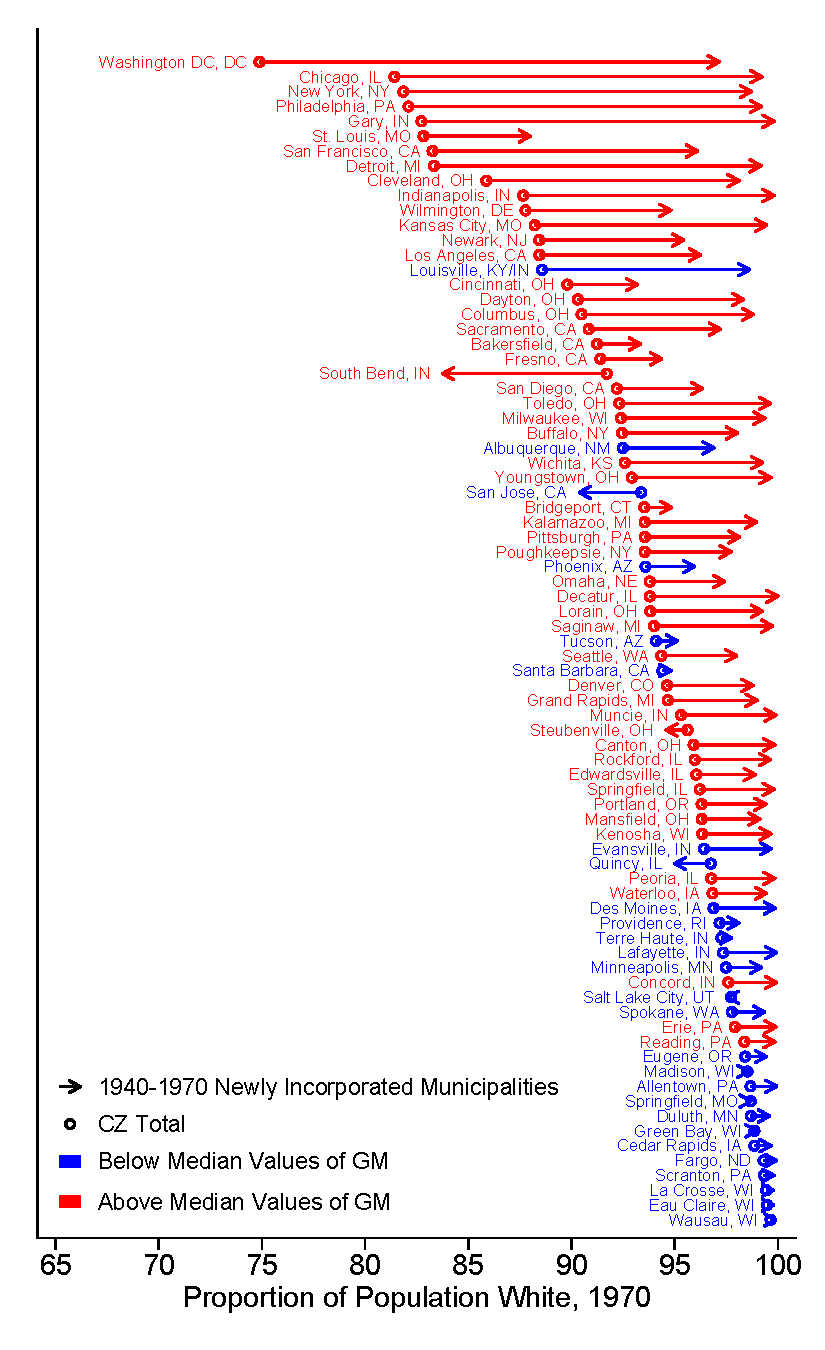
\includegraphics{figures/pcarrow_figure_GM.pdf}
\end{figure}
\clearpage
\begin{figure}
	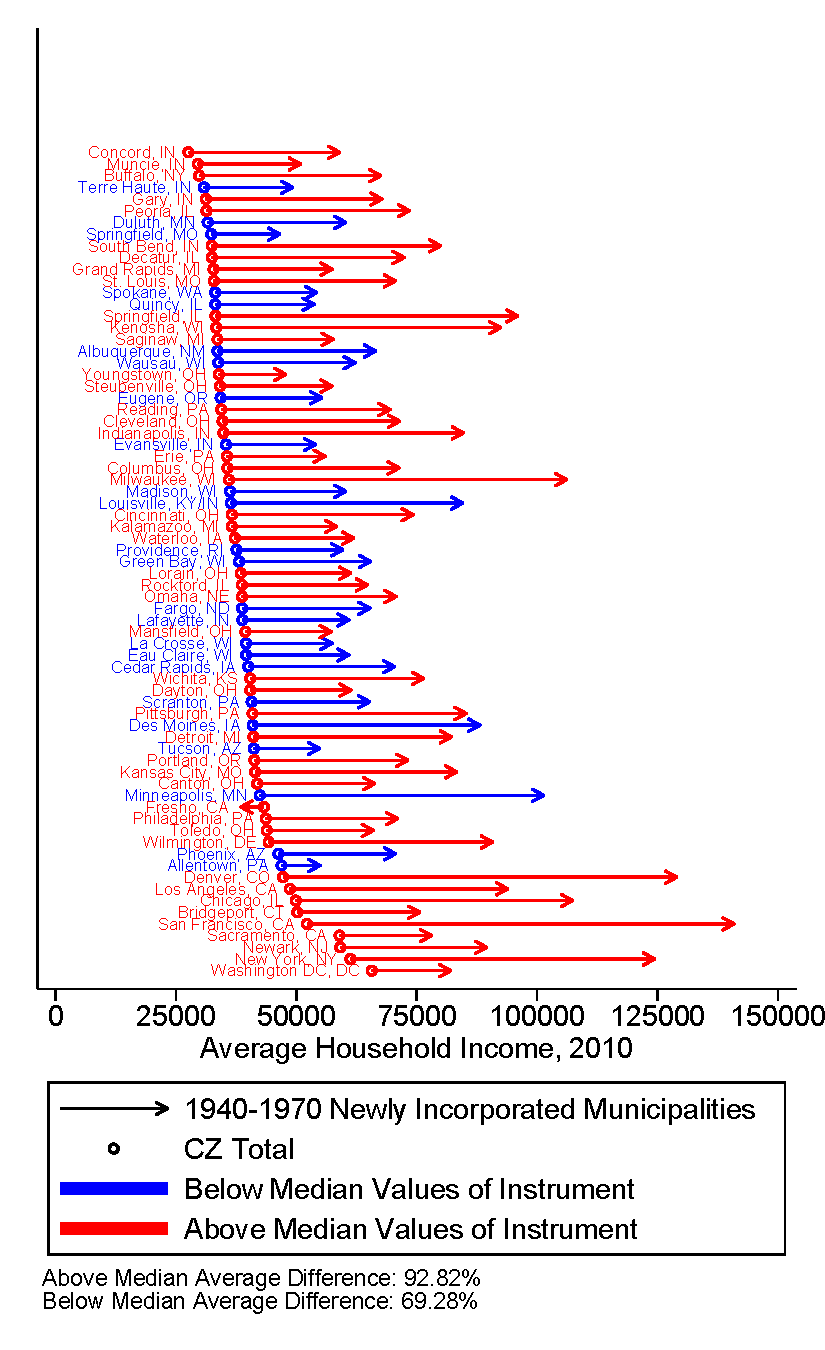
\includegraphics{figures/pcarrow_figure_inc2010.pdf}
\end{figure}
\clearpage
\begin{landscape}
\clearpage
\begin{tabular}{l*{10}{c}} \toprule
&\multicolumn{8}{l}{Panel A: Below Median GM CZs}\\
\cmidrule(lr){1-9}
&\multicolumn{2}{c}{1940-70 Incorporations}&\multicolumn{2}{c}{All other munis}&\multicolumn{2}{c}{Principle Cities}&\multicolumn{2}{c}{CZ Average}\\ \cmidrule(lr){2-3}  \cmidrule(lr){4-5} \cmidrule(lr){6-7} \cmidrule(lr){8-9}
                    &\multicolumn{2}{c}{}     &\multicolumn{2}{c}{}     &\multicolumn{2}{c}{}     &\multicolumn{2}{c}{}     \\
                    &        mean&          sd&        mean&          sd&        mean&          sd&        mean&          sd\\
\midrule
HH Income, 1970     &       12766&        3483&       10884&        1998&       10928&         961&       10249&        1208\\
Home Value, 1970    &    23926.41&     7993.26&    18911.51&     5168.46&    19071.57&     3848.10&    16704.70&     3683.49\\
HH Income, 2010     &    93106.92&    35914.21&    66251.96&    21733.07&    63186.18&    14829.39&    64193.71&    11133.63\\
Pct White, 1970     &       97.46&        4.58&       97.36&        3.03&       95.41&        2.47&       97.57&        2.38\\
Pct White, 2010     &       79.30&       17.70&       82.73&       14.06&       75.24&       14.12&       87.56&        8.02\\
 \toprule
&\multicolumn{8}{l}{Panel B: Above Median GM CZs}\\
\cmidrule(lr){1-9}
&\multicolumn{2}{c}{1940-70 Incorporations}&\multicolumn{2}{c}{All other munis}&\multicolumn{2}{c}{Principle Cities}&\multicolumn{2}{c}{CZ Average}\\ \cmidrule(lr){2-3}  \cmidrule(lr){4-5} \cmidrule(lr){6-7} \cmidrule(lr){8-9}
                    &\multicolumn{2}{c}{}     &\multicolumn{2}{c}{}     &\multicolumn{2}{c}{}     &\multicolumn{2}{c}{}     \\
                    &        mean&          sd&        mean&          sd&        mean&          sd&        mean&          sd\\
\midrule
HH Income, 1970     &       13909&        5272&       12744&        4930&       10899&         922&       11561&        1050\\
Home Value, 1970    &    24188.34&    10264.59&    19825.29&     9170.47&    17723.56&     4297.08&    19469.02&     4371.02\\
HH Income, 2010     &    85549.13&    50883.49&    72903.95&    41440.82&    52307.90&    14353.43&    68475.28&    12857.98\\
Pct White, 1970     &       96.50&       10.70&       96.63&        8.41&       79.97&       13.80&       92.06&        5.41\\
Pct White, 2010     &       80.14&       24.20&       89.44&       16.25&       59.45&       17.34&       79.32&       11.02\\
\toprule
&\multicolumn{8}{l}{Panel C: All CZs}\\
\cmidrule(lr){1-9}
&\multicolumn{2}{c}{1940-70 Incorporations}&\multicolumn{2}{c}{All other munis}&\multicolumn{2}{c}{Principle Cities}&\multicolumn{2}{c}{CZ Average}\\ \cmidrule(lr){2-3}  \cmidrule(lr){4-5} \cmidrule(lr){6-7} \cmidrule(lr){8-9}
                    &\multicolumn{2}{c}{}     &\multicolumn{2}{c}{}     &\multicolumn{2}{c}{}     &\multicolumn{2}{c}{}     \\
                    &        mean&          sd&        mean&          sd&        mean&          sd&        mean&          sd\\
\midrule
HH Income, 1970     &       13673&        5143&       12187&        4595&       10640&         980&        7041&        2498\\
Home Value, 1970    &    23466.38&    10127.76&    18463.10&     8568.00&    17379.00&     3989.75&    11080.05&     4545.15\\
HH Income, 2010     &    82269.09&    48062.29&    68406.05&    35778.02&    53366.29&    12657.06&    55682.89&     9825.92\\
Pct White, 1970     &       96.74&        9.62&       97.19&        7.41&       88.31&       12.97&       94.86&        4.97\\
Pct White, 2010     &       83.55&       21.74&       91.52&       14.13&       71.84&       18.86&       83.86&       10.64\\
\midrule \bottomrule \end{tabular}

\clearpage
\begin{figure}
	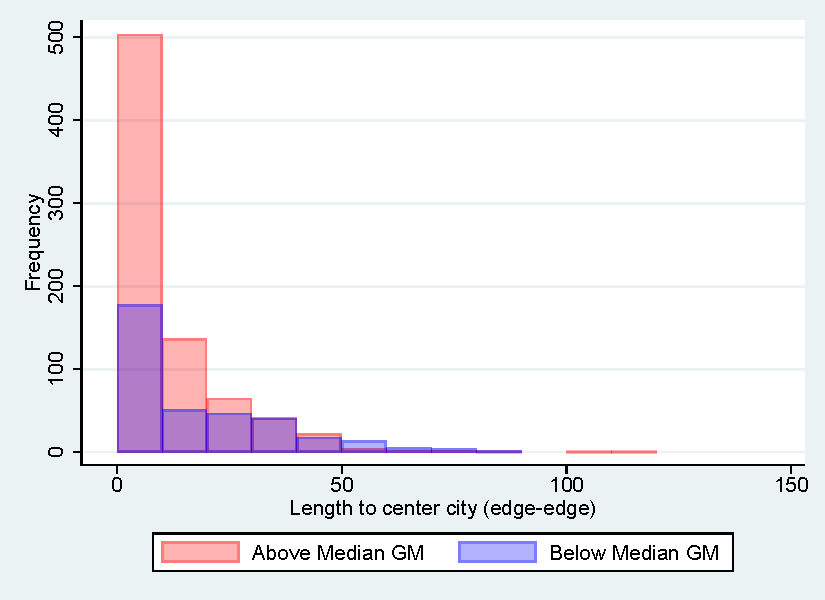
\includegraphics{figures/implications/dist_edge_edge_4070.pdf}
\end{figure}
\clearpage
\begin{figure}
	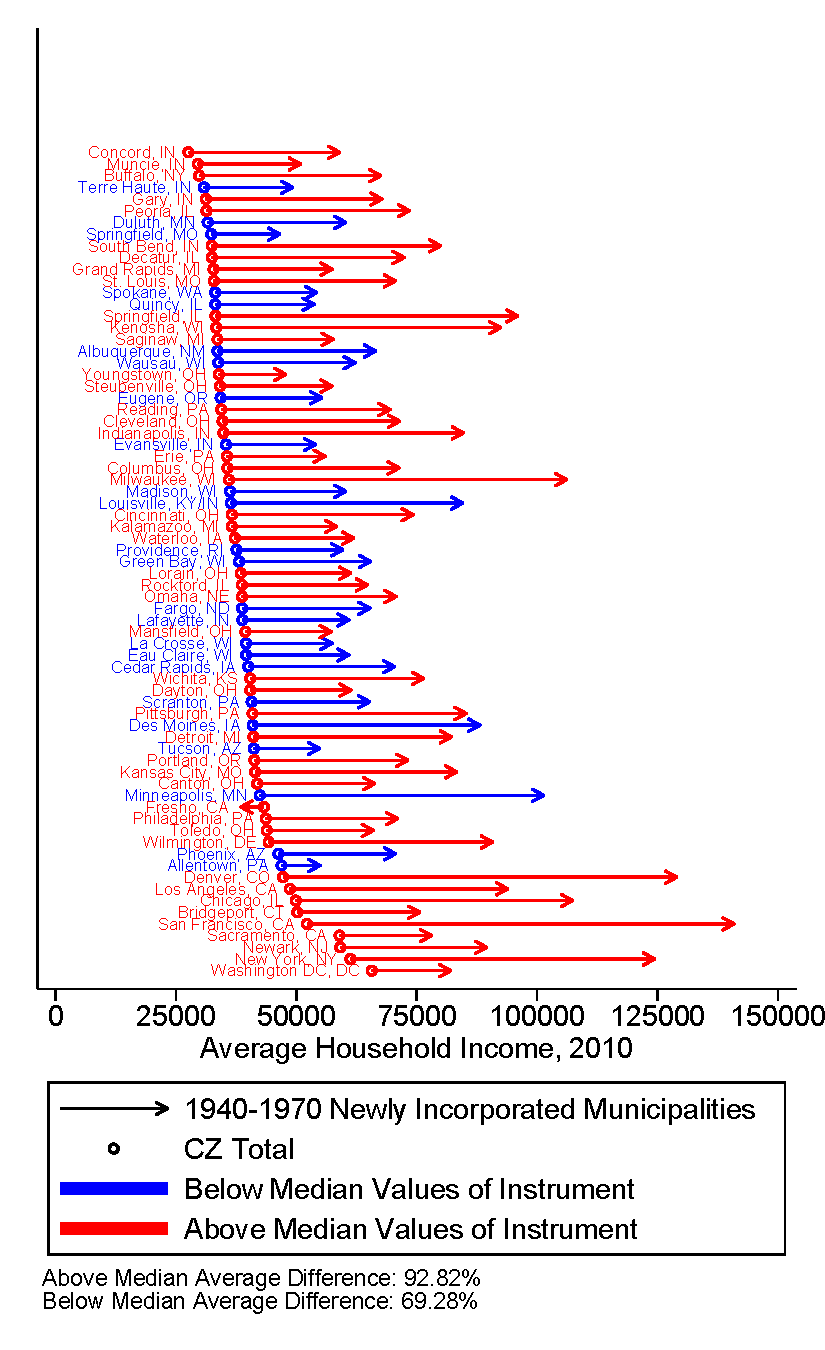
\includegraphics{figures/pcarrow_figure_inc2010.pdf}
\end{figure}
\clearpage
\begin{table}[htbp]\centering
\def\sym#1{\ifmmode^{#1}\else\(^{#1}\)\fi}
\caption{Economic Characteristics}
\begin{tabular}{l*{7}{c}}
\hline\hline
                    &\multicolumn{1}{c}{(1)}&\multicolumn{1}{c}{(2)}&\multicolumn{1}{c}{(3)}&\multicolumn{1}{c}{(4)}&\multicolumn{1}{c}{(5)}&\multicolumn{1}{c}{(6)}&\multicolumn{1}{c}{(7)}\\
                    &\multicolumn{1}{c}{Family Income, 1970}&\multicolumn{1}{c}{Home Value, 1970}&\multicolumn{1}{c}{Household Income, 2010}&\multicolumn{1}{c}{Prop White, 1970}&\multicolumn{1}{c}{Prop White, 2010}&\multicolumn{1}{c}{place\_pop1970}&\multicolumn{1}{c}{Muni Area}\\
\hline
Incorporated 1940-70&    1818.821         &   -1264.950         &    2427.757         &       8.302         &      12.626         &-3244843.865         &  -3.201e+07         \\
                    &  (1990.582)         &  (4979.257)         & (14611.107)         &     (5.095)         &     (9.044)         &(2017697.722)         &(50561626.426)         \\
[1em]
Above Median GM     &     827.587\sym{***}&    2152.461\sym{**} &    2302.127         &      -7.895\sym{***}&     -12.826\sym{***}&  347593.363         &-6268219.456         \\
                    &   (262.536)         &   (894.999)         &  (3416.881)         &     (0.994)         &     (3.085)         &(213280.006)         &(8120199.458)         \\
[1em]
Above Median GM X Inc. 1940-70&    -619.356         &   -2560.180\sym{***}&  -13240.523\sym{***}&       8.309\sym{***}&       9.336\sym{***}& -343132.011         &  -1.694e+07\sym{*}  \\
                    &   (500.678)         &   (969.601)         &  (4255.056)         &     (1.044)         &     (2.044)         &(214640.756)         &(8861990.259)         \\
\hline
Observations        &        2785         &        4251         &        7836         &        4343         &        7836         &        7849         &        7717         \\
\(R^{2}\)           &       0.104         &       0.261         &       0.132         &       0.260         &       0.269         &       0.290         &       0.337         \\
\hline\hline
\multicolumn{8}{l}{\footnotesize Standard errors in parentheses}\\
\multicolumn{8}{l}{\footnotesize \sym{*} \(p<0.10\), \sym{**} \(p<0.05\), \sym{***} \(p<0.01\)}\\
\end{tabular}
\end{table}

\clearpage
\begin{table}[htbp]\centering
\def\sym#1{\ifmmode^{#1}\else\(^{#1}\)\fi}
\caption{Raw Splits}
\begin{tabular}{l*{7}{c}}
\hline\hline
            &\multicolumn{1}{c}{(1)}&\multicolumn{1}{c}{(2)}&\multicolumn{1}{c}{(3)}&\multicolumn{1}{c}{(4)}&\multicolumn{1}{c}{(5)}&\multicolumn{1}{c}{(6)}&\multicolumn{1}{c}{(7)}\\
            &\multicolumn{1}{c}{agg\_fam\_inc\_place1970}&\multicolumn{1}{c}{agg\_house\_value\_place1970}&\multicolumn{1}{c}{mean\_hh\_inc\_place}&\multicolumn{1}{c}{prop\_white1970}&\multicolumn{1}{c}{prop\_white2010}&\multicolumn{1}{c}{place\_pop1970}&\multicolumn{1}{c}{place\_land}\\
\hline
samp\_dest   &    2120.193         &   -5164.475         &   24997.458         &      12.941\sym{***}&       6.369         &-7007869.311\sym{***}&  -4.767e+08\sym{***}\\
            &  (2205.933)         &  (4537.410)         & (17093.031)         &     (3.305)         &    (13.412)         &(618372.385)         & (1.166e+08)         \\
[1em]
above\_x\_med &     -53.621         &      85.399         &   -6464.374\sym{**} &     -11.021\sym{***}&      -4.920         &  668963.747\sym{**} &   2.263e+08\sym{***}\\
            &   (255.675)         &   (693.521)         &  (3257.549)         &     (2.137)         &     (5.302)         &(322438.391)         &(36812344.090)         \\
[1em]
samp\_destXabove\_x\_med&    -322.468         &   -1757.042         &  -10855.403         &      11.235\sym{***}&       1.755         & -658964.189\sym{**} &  -2.453e+08\sym{***}\\
            &   (861.037)         &  (1872.250)         &  (7959.225)         &     (2.010)         &     (4.147)         &(322702.741)         &(36545668.569)         \\
\hline
\(N\)       &         861         &        1020         &        1467         &        1049         &        1467         &        1467         &        1461         \\
\(R^{2}\)   &       0.378         &       0.799         &       0.551         &       0.853         &       0.711         &       0.956         &       0.915         \\
\hline\hline
\multicolumn{8}{l}{\footnotesize Standard errors in parentheses}\\
\multicolumn{8}{l}{\footnotesize \sym{*} \(p<0.10\), \sym{**} \(p<0.05\), \sym{***} \(p<0.01\)}\\
\end{tabular}
\end{table}

\clearpage
\begin{table}[htbp]\centering
\def\sym#1{\ifmmode^{#1}\else\(^{#1}\)\fi}
\caption{Raw Splits}
\begin{tabular}{l*{3}{c}}
\hline\hline
            &\multicolumn{1}{c}{(1)}&\multicolumn{1}{c}{(2)}&\multicolumn{1}{c}{(3)}\\
            &\multicolumn{1}{c}{touching}&\multicolumn{1}{c}{below\_len\_edge}&\multicolumn{1}{c}{len\_edge\_edge}\\
\hline
samp\_dest   &       0.095         &      -0.109         &      -1.050         \\
            &     (0.312)         &     (0.242)         &     (8.510)         \\
[1em]
above\_x\_med &      -0.041         &      -0.040         &       0.465         \\
            &     (0.058)         &     (0.055)         &     (2.342)         \\
[1em]
samp\_destXabove\_x\_med&       0.021         &      -0.023         &       1.852         \\
            &     (0.160)         &     (0.048)         &     (1.927)         \\
\hline
\(N\)       &        8514         &        8514         &        8386         \\
\(R^{2}\)   &       0.038         &       0.072         &       0.085         \\
\hline\hline
\multicolumn{4}{l}{\footnotesize Standard errors in parentheses}\\
\multicolumn{4}{l}{\footnotesize \sym{*} \(p<0.10\), \sym{**} \(p<0.05\), \sym{***} \(p<0.01\)}\\
\end{tabular}
\end{table}

\clearpage
\begin{table}[htbp]\centering
\def\sym#1{\ifmmode^{#1}\else\(^{#1}\)\fi}
\caption{Raw Splits}
\begin{tabular}{l*{4}{c}}
\hline\hline
            &\multicolumn{1}{c}{(1)}&\multicolumn{1}{c}{(2)}&\multicolumn{1}{c}{(3)}&\multicolumn{1}{c}{(4)}\\
            &\multicolumn{1}{c}{exclusive\_district\_place}&\multicolumn{1}{c}{exclusive\_district\_shape}&\multicolumn{1}{c}{psum\_shared\_boundary\_muni}&\multicolumn{1}{c}{min\_hausdorff\_muni}\\
\hline
samp\_dest   &      -0.972\sym{***}&       0.417         &       0.082         &      -0.070\sym{*}  \\
            &     (0.341)         &     (0.287)         &     (0.190)         &     (0.037)         \\
[1em]
above\_x\_med &      -0.042         &      -0.309\sym{*}  &       0.068         &      -0.005         \\
            &     (0.069)         &     (0.166)         &     (0.044)         &     (0.011)         \\
[1em]
samp\_destXabove\_x\_med&       0.209\sym{***}&       0.403\sym{**} &       0.030         &      -0.020\sym{*}  \\
            &     (0.077)         &     (0.167)         &     (0.065)         &     (0.011)         \\
\hline
\(N\)       &        8836         &        8836         &        8836         &        8836         \\
\(R^{2}\)   &       0.163         &       0.480         &       0.166         &       0.446         \\
\hline\hline
\multicolumn{5}{l}{\footnotesize Standard errors in parentheses}\\
\multicolumn{5}{l}{\footnotesize \sym{*} \(p<0.10\), \sym{**} \(p<0.05\), \sym{***} \(p<0.01\)}\\
\end{tabular}
\end{table}

\clearpage
\begin{table}[htbp]\centering
\def\sym#1{\ifmmode^{#1}\else\(^{#1}\)\fi}
\caption{Raw Splits}
\begin{tabular}{l*{4}{c}}
\hline\hline
            &\multicolumn{1}{c}{(1)}&\multicolumn{1}{c}{(2)}&\multicolumn{1}{c}{(3)}&\multicolumn{1}{c}{(4)}\\
            &\multicolumn{1}{c}{exclusive\_district\_place}&\multicolumn{1}{c}{exclusive\_district\_shape}&\multicolumn{1}{c}{psum\_shared\_boundary\_muni}&\multicolumn{1}{c}{min\_hausdorff\_muni}\\
\hline
samp\_dest   &      -1.145\sym{***}&       0.682\sym{**} &      -0.082         &       0.024         \\
            &     (0.309)         &     (0.319)         &     (0.297)         &     (0.057)         \\
[1em]
above\_x\_med &      -0.051         &      -0.369\sym{**} &       0.100\sym{*}  &       0.039\sym{**} \\
            &     (0.089)         &     (0.179)         &     (0.059)         &     (0.017)         \\
[1em]
samp\_destXabove\_x\_med&       0.218\sym{**} &       0.463\sym{**} &      -0.002         &      -0.064\sym{***}\\
            &     (0.104)         &     (0.182)         &     (0.079)         &     (0.016)         \\
\hline
\(N\)       &        1467         &        1467         &        1467         &        1467         \\
\(R^{2}\)   &       0.268         &       0.694         &       0.346         &       0.701         \\
\hline\hline
\multicolumn{5}{l}{\footnotesize Standard errors in parentheses}\\
\multicolumn{5}{l}{\footnotesize \sym{*} \(p<0.10\), \sym{**} \(p<0.05\), \sym{***} \(p<0.01\)}\\
\end{tabular}
\end{table}

\clearpage
\begin{table}[htbp]\centering
\def\sym#1{\ifmmode^{#1}\else\(^{#1}\)\fi}
\caption{Raw Splits}
\begin{tabular}{l*{5}{c}}
\hline\hline
            &\multicolumn{1}{c}{(1)}&\multicolumn{1}{c}{(2)}&\multicolumn{1}{c}{(3)}&\multicolumn{1}{c}{(4)}&\multicolumn{1}{c}{(5)}\\
            &\multicolumn{1}{c}{landuse\_sfr}&\multicolumn{1}{c}{landuse\_apartment}&\multicolumn{1}{c}{pct\_rev\_ff}&\multicolumn{1}{c}{pct\_rev\_sa}&\multicolumn{1}{c}{pct\_rev\_debt}\\
\hline
samp\_dest   &      27.137\sym{**} &      -2.910\sym{***}&       0.018         &       0.809         &      92.093         \\
            &    (11.206)         &     (0.779)         &     (1.078)         &     (1.173)         &   (175.905)         \\
[1em]
above\_x\_med &      -0.751         &       0.619\sym{**} &       0.391\sym{***}&       0.473         &     -61.021\sym{*}  \\
            &     (2.532)         &     (0.270)         &     (0.138)         &     (0.419)         &    (33.267)         \\
[1em]
samp\_destXabove\_x\_med&      10.255\sym{***}&      -0.731\sym{***}&       0.707\sym{**} &      -2.074\sym{***}&      40.542         \\
            &     (2.933)         &     (0.231)         &     (0.309)         &     (0.566)         &    (52.894)         \\
\hline
\(N\)       &        8699         &        8699         &        8694         &        8694         &        8694         \\
\(R^{2}\)   &       0.791         &       0.785         &       0.158         &       0.117         &       0.207         \\
\hline\hline
\multicolumn{6}{l}{\footnotesize Standard errors in parentheses}\\
\multicolumn{6}{l}{\footnotesize \sym{*} \(p<0.10\), \sym{**} \(p<0.05\), \sym{***} \(p<0.01\)}\\
\end{tabular}
\end{table}

\clearpage
\begin{table}[htbp]\centering
\def\sym#1{\ifmmode^{#1}\else\(^{#1}\)\fi}
\caption{Raw Splits}
\begin{tabular}{l*{5}{c}}
\hline\hline
            &\multicolumn{1}{c}{(1)}&\multicolumn{1}{c}{(2)}&\multicolumn{1}{c}{(3)}&\multicolumn{1}{c}{(4)}&\multicolumn{1}{c}{(5)}\\
            &\multicolumn{1}{c}{landuse\_sfr}&\multicolumn{1}{c}{landuse\_apartment}&\multicolumn{1}{c}{pct\_rev\_ff}&\multicolumn{1}{c}{pct\_rev\_sa}&\multicolumn{1}{c}{pct\_rev\_debt}\\
\hline
samp\_dest   &      22.600\sym{*}  &      -3.391\sym{**} &       0.863         &       0.103         &     155.056         \\
            &    (13.016)         &     (1.448)         &     (1.051)         &     (1.398)         &   (174.801)         \\
[1em]
above\_x\_med &      -4.672         &       1.045\sym{**} &       0.502\sym{**} &       0.718\sym{**} &     -83.421\sym{**} \\
            &     (3.155)         &     (0.453)         &     (0.195)         &     (0.282)         &    (38.668)         \\
[1em]
samp\_destXabove\_x\_med&      14.176\sym{***}&      -1.156\sym{***}&       0.596         &      -2.320\sym{***}&      62.942         \\
            &     (3.426)         &     (0.427)         &     (0.399)         &     (0.820)         &    (56.314)         \\
\hline
\(N\)       &        1448         &        1448         &        1439         &        1439         &        1439         \\
\(R^{2}\)   &       0.905         &       0.879         &       0.297         &       0.263         &       0.392         \\
\hline\hline
\multicolumn{6}{l}{\footnotesize Standard errors in parentheses}\\
\multicolumn{6}{l}{\footnotesize \sym{*} \(p<0.10\), \sym{**} \(p<0.05\), \sym{***} \(p<0.01\)}\\
\end{tabular}
\end{table}

\clearpage
\begin{table}[htbp]\centering
\def\sym#1{\ifmmode^{#1}\else\(^{#1}\)\fi}
\caption{Muni-District similarity, CZ level}
\begin{tabular}{l*{4}{c}}
\hline\hline
            &\multicolumn{1}{c}{(1)}&\multicolumn{1}{c}{(2)}&\multicolumn{1}{c}{(3)}&\multicolumn{1}{c}{(4)}\\
            &\multicolumn{1}{c}{EI}&\multicolumn{1}{c}{mean\_dist\_max\_int}&\multicolumn{1}{c}{mean\_min\_hausdorff\_muni}&\multicolumn{1}{c}{mean\_psum\_shared\_muni}\\
\hline
GM\_raw\_pp   &       0.007\sym{***}&       0.011\sym{***}&      -0.004\sym{***}&       0.005         \\
            &     (0.003)         &     (0.003)         &     (0.001)         &     (0.004)         \\
\hline
\(N\)       &         118         &         118         &         118         &         118         \\
\(R^{2}\)   &       0.681         &       0.709         &       0.742         &       0.342         \\
\hline\hline
\multicolumn{5}{l}{\footnotesize Standard errors in parentheses}\\
\multicolumn{5}{l}{\footnotesize \sym{*} \(p<0.10\), \sym{**} \(p<0.05\), \sym{***} \(p<0.01\)}\\
\end{tabular}
\end{table}

\clearpage
\begin{table}[htbp]\centering
\def\sym#1{\ifmmode^{#1}\else\(^{#1}\)\fi}
\caption{Raw Splits}
\begin{tabular}{l*{4}{c}}
\hline\hline
            &\multicolumn{1}{c}{(1)}&\multicolumn{1}{c}{(2)}&\multicolumn{1}{c}{(3)}&\multicolumn{1}{c}{(4)}\\
            &\multicolumn{1}{c}{vr\_blwt\_cz}&\multicolumn{1}{c}{diss\_blwt\_cz}&\multicolumn{1}{c}{SP\_nexpd\_1970}&\multicolumn{1}{c}{rco1970}\\
\hline
GM\_raw\_pp   &       0.016\sym{***}&       0.003\sym{***}&       0.007\sym{***}&      -0.033\sym{***}\\
            &     (0.003)         &     (0.001)         &     (0.002)         &     (0.007)         \\
\hline
\(N\)       &         118         &         118         &         130         &         130         \\
\(R^{2}\)   &       0.724         &       0.582         &       0.258         &       0.433         \\
\hline\hline
\multicolumn{5}{l}{\footnotesize Standard errors in parentheses}\\
\multicolumn{5}{l}{\footnotesize \sym{*} \(p<0.10\), \sym{**} \(p<0.05\), \sym{***} \(p<0.01\)}\\
\end{tabular}
\end{table}

\clearpage
\begin{table}[htbp]\centering
\def\sym#1{\ifmmode^{#1}\else\(^{#1}\)\fi}
\caption{School District Amenities}
\begin{tabular}{l*{5}{c}}
\hline\hline
            &\multicolumn{1}{c}{(1)}&\multicolumn{1}{c}{(2)}&\multicolumn{1}{c}{(3)}&\multicolumn{1}{c}{(4)}&\multicolumn{1}{c}{(5)}\\
            &\multicolumn{1}{c}{mean\_ap}&\multicolumn{1}{c}{totenroll}&\multicolumn{1}{c}{st\_ratio\_leaid}&\multicolumn{1}{c}{pct\_white\_leaid}&\multicolumn{1}{c}{pct\_free\_red\_lunch\_leaid}\\
\hline
int\_0       &      35.346         &    5567.768\sym{*}  &      15.801         &      -2.097\sym{***}&       0.711         \\
            &    (22.336)         &  (3010.331)         &    (12.475)         &     (0.519)         &     (0.708)         \\
[1em]
above\_x\_med &       1.177         &     193.388\sym{**} &       1.910\sym{***}&      -0.087\sym{**} &       0.010         \\
            &     (0.925)         &    (78.164)         &     (0.474)         &     (0.037)         &     (0.022)         \\
[1em]
above\_x\_med\_int\_0&      -4.696         &    -872.194\sym{***}&      -3.359\sym{**} &       0.233\sym{***}&       0.045         \\
            &     (3.479)         &   (324.655)         &     (1.512)         &     (0.074)         &     (0.127)         \\
[1em]
above\_x\_med\_int\_0&       0.000         &       0.000         &       0.000         &       0.000         &       0.000         \\
            &         (.)         &         (.)         &         (.)         &         (.)         &         (.)         \\
\hline
\(N\)       &        3089         &        4224         &        4199         &        4224         &        4224         \\
\(R^{2}\)   &       0.118         &       0.081         &       0.395         &       0.369         &       0.082         \\
\hline\hline
\multicolumn{6}{l}{\footnotesize Standard errors in parentheses}\\
\multicolumn{6}{l}{\footnotesize \sym{*} \(p<0.10\), \sym{**} \(p<0.05\), \sym{***} \(p<0.01\)}\\
\end{tabular}
\end{table}

\clearpage
 \begin{tabular}{l*{9}{c}} \toprule
&\multicolumn{1}{c}{All}&\multicolumn{1}{c}{White}&\multicolumn{1}{c}{Black}&\multicolumn{1}{c}{W-B Gap}&\multicolumn{1}{c}{Not Ec. Disadvantaged}&\multicolumn{1}{c}{Ec. Disadvantaged}&\multicolumn{1}{c}{NEC-ECD Gap}&\\\cmidrule(lr){2-2}\cmidrule(lr){3-3}\cmidrule(lr){4-4}\cmidrule(lr){5-5}\cmidrule(lr){6-6}\cmidrule(lr){7-7}\cmidrule(lr){8-8}
&\multicolumn{1}{c}{(1)}&\multicolumn{1}{c}{(2)}&\multicolumn{1}{c}{(3)}&\multicolumn{1}{c}{(4)}&\multicolumn{1}{c}{(5)}&\multicolumn{1}{c}{(6)}&\multicolumn{1}{c}{(7)}\\
\cmidrule(lr){1-8}
\multicolumn{7}{l}{Panel A: IV with GM}\\
\cmidrule(lr){1-8}
Percentage Point Change in Urban Black Population&   -0.003   &    0.002   &   -0.001   &    0.003   &   -0.002   &   -0.003** &    0.001   \\
                &  (0.002)   &  (0.004)   &  (0.002)   &  (0.003)   &  (0.002)   &  (0.001)   &  (0.002)   \\
\cmidrule(lr){1-8}
\multicolumn{7}{l}{Panel B: OLS with Munis}\\
\cmidrule(lr){1-8}
New Number of Municipal Govts, P.C. (total)&   -0.114** &    0.083   &   -0.010   &    0.079   &    0.010   &   -0.040   &    0.046   \\
                &  (0.047)   &  (0.077)   &  (0.039)   &  (0.072)   &  (0.049)   &  (0.037)   &  (0.054)   \\
\cmidrule(lr){1-8}
\multicolumn{7}{l}{Panel C: Two Step with Munis}\\
\cmidrule(lr){1-8}
New Number of Municipal Govts, P.C. (total)&   -0.493** &   -0.098   &   -0.404** &    0.244   &   -0.454** &   -0.498***&    0.032   \\
                &  (0.198)   &  (0.333)   &  (0.156)   &  (0.246)   &  (0.213)   &  (0.131)   &  (0.168)   \\
\midrule
Dep. Var Mean   &    0.045   &    0.180   &   -0.377   &    0.562   &    0.318   &   -0.255   &    0.574   \\
Observations    &      130   &      130   &      130   &      130   &      130   &      130   &      130   \\
\cmidrule(lr){1-8}
\multicolumn{7}{l}{Panel B: OLS with School Districts}\\
\cmidrule(lr){1-8}
New Ind. Sch. Dists., P.C. (total)&    0.001   &    0.006***&    0.003** &    0.002   &    0.002*  &    0.001   &    0.001   \\
                &  (0.002)   &  (0.002)   &  (0.001)   &  (0.002)   &  (0.001)   &  (0.001)   &  (0.002)   \\
\cmidrule(lr){1-8}
\multicolumn{7}{l}{Panel E: Two Step with School Districts}\\
\cmidrule(lr){1-8}
New Ind. Sch. Dists., P.C. (total)&   -0.005** &   -0.001   &   -0.004** &    0.001   &   -0.007** &   -0.007***&   -0.001   \\
                &  (0.003)   &  (0.005)   &  (0.002)   &  (0.005)   &  (0.003)   &  (0.002)   &  (0.003)   \\
\midrule
Dep. Var Mean   &    0.039   &    0.174   &   -0.390   &    0.570   &    0.313   &   -0.258   &    0.572   \\
Observations    &      118   &      118   &      118   &      118   &      118   &      118   &      118   \\
       \bottomrule \end{tabular}

\clearpage
\begin{table}[htbp]\centering
\def\sym#1{\ifmmode^{#1}\else\(^{#1}\)\fi}
\caption{School District Capital Expenditure}
\begin{tabular}{l*{4}{c}}
\hline\hline
                    &\multicolumn{1}{c}{(1)}&\multicolumn{1}{c}{(2)}&\multicolumn{1}{c}{(3)}&\multicolumn{1}{c}{(4)}\\
                    &\multicolumn{1}{c}{Capital outlays/Total Expenditure}&\multicolumn{1}{c}{Capital outlays/Total Enrollment}&\multicolumn{1}{c}{Log Capital Outlays}&\multicolumn{1}{c}{log(Capital outlays/Total Enrollment)}\\
\hline
Prop Border with 40-70 incorporation&       0.040         &       1.275         &       2.175         &       1.288         \\
                    &     (0.088)         &  (1318.729)         &     (2.454)         &     (1.254)         \\
[1em]
Above Median GM     &      -0.002         &      73.278         &       0.516\sym{**} &       0.137         \\
                    &     (0.009)         &   (105.966)         &     (0.214)         &     (0.104)         \\
[1em]
Prop Border 40-70 X Above Median GM&      -0.036         &    -385.582         &      -1.882\sym{***}&      -0.520\sym{**} \\
                    &     (0.022)         &   (364.857)         &     (0.496)         &     (0.244)         \\
\hline
Observations        &        4117         &        4117         &        4116         &        4116         \\
\(R^{2}\)           &       0.063         &       0.013         &       0.180         &       0.055         \\
\hline\hline
\multicolumn{5}{l}{\footnotesize Standard errors in parentheses}\\
\multicolumn{5}{l}{\footnotesize \sym{*} \(p<0.10\), \sym{**} \(p<0.05\), \sym{***} \(p<0.01\)}\\
\end{tabular}
\end{table}

\clearpage
\begin{table}[htbp]\centering
\def\sym#1{\ifmmode^{#1}\else\(^{#1}\)\fi}
\caption{Raw Splits}
\begin{tabular}{l*{7}{c}}
\hline\hline
            &\multicolumn{1}{c}{(1)}&\multicolumn{1}{c}{(2)}&\multicolumn{1}{c}{(3)}&\multicolumn{1}{c}{(4)}&\multicolumn{1}{c}{(5)}&\multicolumn{1}{c}{(6)}&\multicolumn{1}{c}{(7)}\\
            &\multicolumn{1}{c}{mf}&\multicolumn{1}{c}{mixed\_use}&\multicolumn{1}{c}{attached\_sfr}&\multicolumn{1}{c}{adu}&\multicolumn{1}{c}{flex\_zoning\_br}&\multicolumn{1}{c}{min\_lot\_size\_mean}&\multicolumn{1}{c}{min\_lot\_size\_max}\\
\hline
samp\_dest   &      -0.094         &      -0.831         &      -0.760\sym{***}&      -1.184\sym{**} &      -0.154         &   49889.752\sym{**} &  139634.815         \\
            &     (0.082)         &     (0.557)         &     (0.196)         &     (0.596)         &     (0.248)         & (23167.306)         & (84248.118)         \\
[1em]
above\_x\_med &      -0.000         &      -0.128\sym{***}&       0.384\sym{***}&       0.093         &       0.189         &   -7415.561         &  -53398.490\sym{*}  \\
            &     (0.004)         &     (0.040)         &     (0.130)         &     (0.125)         &     (0.136)         &  (6868.233)         & (31694.361)         \\
[1em]
samp\_destXabove\_x\_med&       0.002         &       0.037         &      -0.411\sym{***}&      -0.228\sym{*}  &      -0.227         &   -2933.187         &   46993.519         \\
            &     (0.008)         &     (0.090)         &     (0.096)         &     (0.137)         &     (0.163)         &  (9744.735)         & (33741.665)         \\
\hline
\(N\)       &        3349         &        3326         &        3401         &        3383         &        3402         &        3156         &        3150         \\
\(R^{2}\)   &       0.008         &       0.086         &       0.382         &       0.321         &       0.192         &       0.228         &       0.230         \\
\hline\hline
\multicolumn{8}{l}{\footnotesize Standard errors in parentheses}\\
\multicolumn{8}{l}{\footnotesize \sym{*} \(p<0.10\), \sym{**} \(p<0.05\), \sym{***} \(p<0.01\)}\\
\end{tabular}
\end{table}

\clearpage
\begin{table}[htbp]\centering
\def\sym#1{\ifmmode^{#1}\else\(^{#1}\)\fi}
\caption{Raw Splits}
\begin{tabular}{l*{7}{c}}
\hline\hline
            &\multicolumn{1}{c}{(1)}&\multicolumn{1}{c}{(2)}&\multicolumn{1}{c}{(3)}&\multicolumn{1}{c}{(4)}&\multicolumn{1}{c}{(5)}&\multicolumn{1}{c}{(6)}&\multicolumn{1}{c}{(7)}\\
            &\multicolumn{1}{c}{mf}&\multicolumn{1}{c}{mixed\_use}&\multicolumn{1}{c}{attached\_sfr}&\multicolumn{1}{c}{adu}&\multicolumn{1}{c}{flex\_zoning\_br}&\multicolumn{1}{c}{min\_lot\_size\_mean}&\multicolumn{1}{c}{min\_lot\_size\_max}\\
\hline
samp\_dest   &      -0.090         &      -0.901         &      -0.978\sym{***}&      -1.774\sym{***}&      -0.047         &   82017.323\sym{**} &  290103.876\sym{*}  \\
            &         (.)         &     (0.581)         &     (0.298)         &     (0.562)         &     (0.402)         & (37780.021)         &(156098.843)         \\
[1em]
above\_x\_med &       0.000         &      -0.039         &       0.507\sym{***}&      -0.066         &       0.521\sym{**} &  -11133.497         &  -89893.176\sym{**} \\
            &         (.)         &     (0.034)         &     (0.159)         &     (0.135)         &     (0.231)         &  (8007.805)         & (37177.727)         \\
[1em]
samp\_destXabove\_x\_med&       0.002         &      -0.052         &      -0.534\sym{***}&      -0.069         &      -0.559\sym{**} &     784.748         &   83488.202\sym{**} \\
            &         (.)         &     (0.099)         &     (0.143)         &     (0.163)         &     (0.251)         & (10460.136)         & (39702.217)         \\
\hline
\(N\)       &         765         &         735         &         776         &         773         &         774         &         705         &         699         \\
\(R^{2}\)   &       0.029         &       0.306         &       0.637         &       0.531         &       0.496         &       0.471         &       0.433         \\
\hline\hline
\multicolumn{8}{l}{\footnotesize Standard errors in parentheses}\\
\multicolumn{8}{l}{\footnotesize \sym{*} \(p<0.10\), \sym{**} \(p<0.05\), \sym{***} \(p<0.01\)}\\
\end{tabular}
\end{table}

\clearpage
\begin{table}[htbp]\centering
\def\sym#1{\ifmmode^{#1}\else\(^{#1}\)\fi}
\caption{AI Zoning - Regulations}
\begin{tabular}{l*{5}{c}}
\hline\hline
                    &\multicolumn{1}{c}{(1)}&\multicolumn{1}{c}{(2)}&\multicolumn{1}{c}{(3)}&\multicolumn{1}{c}{(4)}&\multicolumn{1}{c}{(5)}\\
                    &\multicolumn{1}{c}{Inclusionary Zoning}&\multicolumn{1}{c}{Permit caps}&\multicolumn{1}{c}{Number of agencies}&\multicolumn{1}{c}{Public hearings for MF}&\multicolumn{1}{c}{Max review days}\\
\hline
Incorporated 1940-70&       0.301         &       0.903\sym{***}&      -1.248\sym{*}  &       0.601\sym{*}  &     -82.383         \\
                    &     (0.356)         &     (0.299)         &     (0.644)         &     (0.334)         &    (93.938)         \\
[1em]
Above Median GM     &       0.179\sym{*}  &       0.004         &      -0.194         &       0.130         &      68.079\sym{***}\\
                    &     (0.106)         &     (0.059)         &     (0.159)         &     (0.085)         &    (22.275)         \\
[1em]
Above Median GM X Inc. 1940-70&      -0.502\sym{***}&      -0.005         &       0.963\sym{***}&      -0.083         &     -34.216         \\
                    &     (0.089)         &     (0.060)         &     (0.222)         &     (0.102)         &    (31.136)         \\
\hline
Observations        &        2520         &        2637         &        2613         &        2599         &        2311         \\
\(R^{2}\)           &       0.215         &       0.047         &       0.068         &       0.048         &       0.108         \\
\hline\hline
\multicolumn{6}{l}{\footnotesize Standard errors in parentheses}\\
\multicolumn{6}{l}{\footnotesize \sym{*} \(p<0.10\), \sym{**} \(p<0.05\), \sym{***} \(p<0.01\)}\\
\end{tabular}
\end{table}

\clearpage
\begin{table}[htbp]\centering
\def\sym#1{\ifmmode^{#1}\else\(^{#1}\)\fi}
\caption{Raw Splits}
\begin{tabular}{l*{6}{c}}
\hline\hline
            &\multicolumn{1}{c}{(1)}&\multicolumn{1}{c}{(2)}&\multicolumn{1}{c}{(3)}&\multicolumn{1}{c}{(4)}&\multicolumn{1}{c}{(5)}&\multicolumn{1}{c}{(6)}\\
            &\multicolumn{1}{c}{mf\_conversion\_allowed}&\multicolumn{1}{c}{inclusionary\_zoning}&\multicolumn{1}{c}{permit\_cap\_phasing}&\multicolumn{1}{c}{n\_approving\_agencies}&\multicolumn{1}{c}{mf\_public\_hearing}&\multicolumn{1}{c}{max\_review\_days}\\
\hline
samp\_dest   &      -0.576\sym{**} &      -0.256         &      -0.086         &      -1.141         &       0.580         &      30.721         \\
            &     (0.248)         &     (0.430)         &     (0.343)         &     (1.308)         &     (0.463)         &   (145.700)         \\
[1em]
above\_x\_med &      -0.590\sym{***}&       0.775\sym{***}&       0.470\sym{**} &      -0.510         &       0.583\sym{***}&     448.583\sym{***}\\
            &     (0.122)         &     (0.133)         &     (0.180)         &     (0.367)         &     (0.161)         &   (101.521)         \\
[1em]
samp\_destXabove\_x\_med&       0.616\sym{***}&      -1.060\sym{***}&      -0.464\sym{**} &       1.223\sym{***}&      -0.491\sym{***}&    -425.757\sym{***}\\
            &     (0.134)         &     (0.171)         &     (0.188)         &     (0.395)         &     (0.146)         &   (105.259)         \\
\hline
\(N\)       &         774         &         743         &         776         &         764         &         760         &         676         \\
\(R^{2}\)   &       0.865         &       0.754         &       0.528         &       0.575         &       0.534         &       0.724         \\
\hline\hline
\multicolumn{7}{l}{\footnotesize Standard errors in parentheses}\\
\multicolumn{7}{l}{\footnotesize \sym{*} \(p<0.10\), \sym{**} \(p<0.05\), \sym{***} \(p<0.01\)}\\
\end{tabular}
\end{table}

\clearpage
\begin{table}[htbp]\centering
\def\sym#1{\ifmmode^{#1}\else\(^{#1}\)\fi}
\caption{Raw Splits}
\begin{tabular}{l*{7}{c}}
\hline\hline
            &\multicolumn{1}{c}{(1)}&\multicolumn{1}{c}{(2)}&\multicolumn{1}{c}{(3)}&\multicolumn{1}{c}{(4)}&\multicolumn{1}{c}{(5)}&\multicolumn{1}{c}{(6)}&\multicolumn{1}{c}{(7)}\\
            &\multicolumn{1}{c}{age\_restrictions}&\multicolumn{1}{c}{inclusionary\_zoning\_comply}&\multicolumn{1}{c}{lot\_size\_nature\_restriction}&\multicolumn{1}{c}{max\_frontage\_req\_sfr}&\multicolumn{1}{c}{n\_steps\_mf}&\multicolumn{1}{c}{First\_PC}&\multicolumn{1}{c}{Second\_PC}\\
\hline
samp\_dest   &       0.261         &       0.157         &      -0.077         &      84.956         &      -1.577         &      -0.863         &       2.046\sym{***}\\
            &     (0.842)         &     (0.142)         &     (0.268)         &    (56.563)         &     (1.665)         &     (1.455)         &     (0.643)         \\
[1em]
above\_x\_med &       0.562\sym{***}&       0.059         &       0.011         &       4.612         &       0.235         &       1.726\sym{***}&      -0.356\sym{*}  \\
            &     (0.093)         &     (0.037)         &     (0.030)         &    (12.399)         &     (0.247)         &     (0.512)         &     (0.196)         \\
[1em]
samp\_destXabove\_x\_med&      -0.603\sym{***}&      -0.170\sym{***}&      -0.017         &     -23.377         &      -0.043         &      -2.475\sym{***}&       0.231         \\
            &     (0.162)         &     (0.051)         &     (0.063)         &    (16.974)         &     (0.387)         &     (0.395)         &     (0.249)         \\
\hline
\(N\)       &        3068         &        3397         &        2816         &        3060         &        3391         &        3405         &        3405         \\
\(R^{2}\)   &       0.364         &       0.100         &       0.060         &       0.399         &       0.151         &       0.286         &       0.405         \\
\hline\hline
\multicolumn{8}{l}{\footnotesize Standard errors in parentheses}\\
\multicolumn{8}{l}{\footnotesize \sym{*} \(p<0.10\), \sym{**} \(p<0.05\), \sym{***} \(p<0.01\)}\\
\end{tabular}
\end{table}

\clearpage
\begin{table}[htbp]\centering
\def\sym#1{\ifmmode^{#1}\else\(^{#1}\)\fi}
\caption{Raw Splits}
\begin{tabular}{l*{7}{c}}
\hline\hline
            &\multicolumn{1}{c}{(1)}&\multicolumn{1}{c}{(2)}&\multicolumn{1}{c}{(3)}&\multicolumn{1}{c}{(4)}&\multicolumn{1}{c}{(5)}&\multicolumn{1}{c}{(6)}&\multicolumn{1}{c}{(7)}\\
            &\multicolumn{1}{c}{age\_restrictions}&\multicolumn{1}{c}{inclusionary\_zoning\_comply}&\multicolumn{1}{c}{lot\_size\_nature\_restriction}&\multicolumn{1}{c}{max\_frontage\_req\_sfr}&\multicolumn{1}{c}{n\_steps\_mf}&\multicolumn{1}{c}{First\_PC}&\multicolumn{1}{c}{Second\_PC}\\
\hline
samp\_dest   &       0.317         &       0.334         &      -0.179         &      72.126         &      -3.326\sym{*}  &      -1.877         &       2.852\sym{***}\\
            &     (0.763)         &     (0.229)         &     (0.228)         &    (69.967)         &     (1.991)         &     (1.272)         &     (0.888)         \\
[1em]
above\_x\_med &       0.790\sym{***}&       0.094         &       0.035         &       9.632         &       0.966\sym{**} &       2.783\sym{***}&      -0.645\sym{**} \\
            &     (0.101)         &     (0.120)         &     (0.046)         &    (19.832)         &     (0.382)         &     (0.461)         &     (0.269)         \\
[1em]
samp\_destXabove\_x\_med&      -0.831\sym{***}&      -0.205         &      -0.040         &     -28.398         &      -0.774         &      -3.533\sym{***}&       0.520\sym{*}  \\
            &     (0.163)         &     (0.130)         &     (0.080)         &    (24.575)         &     (0.514)         &     (0.406)         &     (0.301)         \\
\hline
\(N\)       &         714         &         775         &         647         &         718         &         775         &         776         &         776         \\
\(R^{2}\)   &       0.670         &       0.213         &       0.122         &       0.576         &       0.400         &       0.689         &       0.484         \\
\hline\hline
\multicolumn{8}{l}{\footnotesize Standard errors in parentheses}\\
\multicolumn{8}{l}{\footnotesize \sym{*} \(p<0.10\), \sym{**} \(p<0.05\), \sym{***} \(p<0.01\)}\\
\end{tabular}
\end{table}

\end{landscape}

\end{document}
